\documentclass[letterpaper, 10pt]{article}
\usepackage[margin=2cm]{geometry}
\usepackage{graphicx}
\usepackage{float}
\usepackage{placeins}


% Table de contenidos clickeable
\usepackage{hyperref}
\hypersetup{
	colorlinks,
	citecolor=black,
	filecolor=black,
	linkcolor=black,
	urlcolor=black
}

% Localización
\usepackage[spanish]{babel}
\addto\captionsspanish{
    \renewcommand{\tablename}{Tabla}
    \renewcommand{\listtablename}{Índice de tablas} % Change to "Tablas" if you prefer
}
% Números de páginas
\pagenumbering{arabic}
\usepackage{fancyhdr}
\pagestyle{fancy}
\fancyhf{}
\renewcommand{\headrulewidth}{0pt}
\fancyhead[R]{\thepage}

%

% Ambiente para las listas de la portada
\newenvironment{simplelist}
	{
		\renewcommand\labelitemi{}
		\begin{itemize}
		\setlength{\itemsep}{0pt}
		\setlength{\parskip}{0pt}
	}
	{\end{itemize}}

%

\begin{document}

\begin{titlepage}

\begin{center}
	{\bf Universidad de Santiago de Chile}
	\\
    {\bf Facultad de Ciencia}
	\\
    {\bf Departamento de Matem\'atica y Ciencia de la Computaci\'on}
\end{center}

%

\vfill
\begin{center}
{\large\bf Ingeniería de Software II}
\\
{\Large\bf Informe Nº3. “Análisis Orientado a Objetos OMT++”}\\
\vspace{1cm}
{\Huge\bf Snoozefest}\\
\vspace{2cm}

\includegraphics[height=200pt,width=200pt]{./logo.png}
\end{center}
\vfill

%

\begin{flushright}
	\begin{minipage}{0.3\textwidth}
		Integrantes:
		\begin{simplelist}
			\item Gabriel Carrillo
			\item Erick Aranda
			\item Jose Cuellar
			\item Elías Gangas
			\item Vicente Rojas
		\end{simplelist}
	

		Profesor:
		\begin{simplelist}
			\item Dino Araya
		\end{simplelist}
	
		Fecha de entrega:
		\begin{simplelist}
			\item 27 de noviembre del 2024
		\end{simplelist}
	\end{minipage}
\end{flushright}

\end{titlepage}


{\centering\tableofcontents\par}
{\centering\listoftables\par}
{\centering\listoffigures\par}
\clearpage

\section{Introducción}

En el presente informe el equipo organiza las principales ideas obtenidas durante el avance anterior. Se capturan los requerimientos funcionales, no funcionales, y de implementación. A partir de estos se crea el diagrama de casso de uso UML y se especifican los casos de uso no triviales, es decir, aquellos cuya complejidad no ameritan una especificación detallada. En la especificación, se describe el flujo de normal de dichos casos de uso, además de las excepciones que puedan ocurrir durante ellos.

\section{Objetivos del Proyecto}
En esta sección se presenta el objetivo general y los objetivos específicos para el correcto desarrollo e implementación de Snoozefest.
\subsection{Objetivo General}
Diseñar e implementar la aplicación móvil Snoozefest, una aplicación de alarmas que requieren la solución de desafíos para ser desactivadas.
\subsection{Objetivos Específicos}
A continuación se detallan los objetivos específicos que se consideran hitos claves para el desarrollo del proyecto con metodología ágil.
\begin{itemize}
	\item Anteproyecto y planificación.
	\item Análisis de requerimientos (Historias de usuario).
	\item Análisis orientado a objetos (AOO).
	\item Diseño orientado a objetos (DOO).
	\item Programación orientada a objetos (POO).
	\item Pruebas de programación.
	\item Pruebas de aceptación.
	\item Puesta en producción.
\end{itemize}

\section{Descripción de la Problemática}
En esta sección se da a conocer la motivación y el enfoque del proyecto, además de las soluciones actualmente presentes a la problemática.

\subsection{Motivación}
Muchas personas presentan dificultades para despertar con alarmas tradicionales. Esto puede deberse a diversos factores, como trastornos del sueño, factores ambientales, o simplemente variaciones normales entre individuos. Frecuentemente, las alarmas tradicionales son desactivadas por dichas personas mientras se encuentran en un estado de ``inercia del sueño", una etapa entre el sueño y la vigilia en que el individuo experimenta capacidad cognitiva limitada.
\\
Una solución actualmente aplicada a esta problemática es el uso de desafíos cognitivos que deber ser resueltos antes de desactivar las alarmas. Si bien esto puede dar buenos resultados, no se trata de una solución completa. Por ejemplo, no considera que la severidad de la inercia del sueño varía entre un día y otro incluso para un mismo individuo, y por lo tanto también debería variar la dificultad de los desafíos presentados. Si bien existe la posibilidad de establecer múltiples alarmas manualmente, esto presenta de la dificultad adicional de organizar manualmente dichas alarmas y sus dificultades, lo cual se dificulta aún más por los horarios de sueño irregulares presentados por personas con trastornos del sueño.
\\
Este proyecto busca desarrollar una solución completa a esta problemática, permitiendo que es usuario pueda establecer fácilmente conjuntos de alarmas cuyos desafíos se ajusten a sus necesidades personales.

\subsection{Definición del Problema}
El problema esta en que normalmente tenemos aplicaciones predeterminadas, las cuales ocupamos para poner nuestras alarmas para poder despertar, ese es el uso común de estas, pero en mas de un caso se da, que inconscientemente desactivamos esta alarma por el motivo que sea, pero seguido de esto no tenemos nada mas que nos pueda despertar, y la gente tiende a poner mas de una alarma consecutiva para que en el caso que se desactive esta misma, vuelva a sonar otra dentro de un periodo de tiempo.
\subsection{Estado del Arte}
	Las siguientes aplicaciones de alarmas ocupan nichos similares en la tienda de aplicaciones de Android.

	\begin{enumerate}
		\item[] \textbf{Alarmy:} Permite establecer alarmas con desafíos aritméticos, entre otros.
		\item[] \textbf{Walk Me Up:} Requiere que el usuario camine una cierta cantidad de pasos para desactivar la alarma.
		\item[] \textbf{AMdroid:} Permite establecer distintos desafíos, entre otras configuraciones.
	\end{enumerate}

\section{Descripción de la Solución Propuesta}
En esta sección se detalla la solución propuesta a la problemática anteriormente definida. Se presentan las características, propósitos, alcances, y limitaciones de esta.
\subsection{Características de la Solución}
Las caracteristicas de la solución son las siguientes:

\begin{itemize}
    \item Configución de alarmas: El sistema permite configurar distintas alarmas.
    \item Desafíos para desactivar alarmas: El sistema incluira distintos desafios para poder desactivar la alarma (aritmeticos/puzzle).
    \item Dificultades de los desafíos: El sistema contendra distintos niveles de dificultad.
    \item Configuración de alarmas por intervalo: El usuario puede configurar una serie de alarmas que suenan entre un intervalo de tiempo definido y cuyos desafíos son incrementalmente más difíciles.
\end{itemize}
\subsection{Propósitos de la Solución}
La solución propuesta consiste en el desarrollo de una aplicación de alarmas innovadora que ofrece un método de despertar más efectivo y personalizado. Esta aplicación permitirá a los usuarios configurar alarmas, integrando ejercicios mentales como retos cognitivos que deben completar para desactivar la alarma. Al incorporar esta funcionalidad, se busca fomentar la actividad cerebral y asegurar un despertar más activo y consciente. Además, la aplicación recopilará datos comportamientos de los usuarios, lo que permitirá disminuir la dificultad o aumentar según el tiempo que demore en desactivar la alarma, garantizando así una experiencia de despertar más satisfactoria, efectiva y entretenida.
 
\begin{itemize}
    \item Experiencia usuario: Ofrecer un método de despertar que se adapte a las necesidades individuales de los usuarios, proporcionando una herramienta que garantice un despertar más activo y entretenido.
    \item Activación cerebral: Incorporar ejercicios cognitivos que desafíen la mente del usuario, promoviendo una mayor agilidad mental desde el momento del despertar.
    \item Obtención de datos: Recopilar información sobre el comportamiento de los usuarios con el fin de aumentar o disminuir la dificultad de los retos, mejorando la personalización de la experiencia.
\end{itemize}

\subsection{Alcances y Limitaciones de la Solución}
\begin{itemize}
    \item \textbf{Alcances:}
    \begin{itemize}
        \item Realización de una aplicación móvil para crear alarmas personalizadas con desafios de distintas dificultades.
        \item  Entrega de documentación técnica, documentación de código y manual de usuario.
    \end{itemize}
    \item \textbf{Limitaciones:}
     \begin{itemize}
        \item La aplicación solo se podrá utilizar en un dispositivo móvil Android.
        \item La aplicación solo estara disponible en español.
    \end{itemize}
    
\end{itemize}

\section{Metodología, Herramientas, y Ambiente de Desarrollo}
En esta sección se describirán las metodologías que se usarán para gestionar el ciclo de vida del proyecto. Además, se detallarán las herramientas y el ambiente de desarrollo en que se trabajará.
\subsection{Metodología a Usar}
Para el proyecto se utilizará la metodología ágil SCRUM\cite{1}. Esta metodología fue desarrollada por los desarrolladores de software Ken Schwaber y Jeff Sutherland. El marco de trabajo Scrum consiste en los Equipos Scrum y sus roles, eventos, artefactos y reglas asociadas\cite{2}. Cada componente dentro del marco de trabajo sirve para un propósito específico y es esencial para el éxito de Scrum. El propósito de utilizar esta metodología es que al ser ágil nos ofrece una adaptabilidad a los requisitos, además que nos ofrece adaptabilidad a los requisitos y fomenta la colaboración continua entre los miembros del equipo. Esto permite responder de manera rápida a los cambios en el entorno del proyecto y a las necesidades del cliente, lo que a su vez contribuye a la entrega de productos de alta calidad en ciclos de desarrollo cortos.
\subsection{Herramientas de Desarrollo}
%Tabla de hardware y software
\subsubsection{Hardware}
Para este proyecto se cuenta con 6 computadores personales y 1 teléfono celular de prueba como se muestra en la tabla 
\ref{table:1}.
\begin{table}[H]
    \centering
    \caption{Hardware}
	\vspace{0.2cm}
    \begin{tabular}{|c|c|c|c|c|} \hline
        \textbf{PC} & \textbf{Procesador} & \textbf{Ram} & \textbf{Sistema operativo} & \textbf{Propósito}  \\ \hline
         PC1 & Intel Core i5-10300H       & 16 GB        & Windows 11 & Desarrollo \\\hline
         PC2 & Ryzen 5 2600x       &  16GB      & Windows 10 & Desarrollo\\\hline
         PC3 & Ryzen 7 4800H       &  16GB      & Windows 11  & Pruebas\\\hline
         PC4 & Ryzen 7 4800H       &  16GB      & Windows 11 & Desarrollo y Pruebas\\\hline
		 PC5 & Intel Core i5-4690k &  16GB		& Arch Linux & Desarrollo y Pruebas\\\hline
		 PC6 & MacBook Air 2015	   &  4GB		& Arch Linux & Desarrollo\\\hline
		 Celular1 &	POCO M4 Pro 5G &  6GB		& Android	 & Pruebas\\\hline
    \end{tabular}
    
    \label{table:1}
\end{table}
\newpage
\subsubsection{Software}
%Profundizar en el uso del software visual studio, mysql, php, etc etc
Para el software se contarán con los siguientes programas especificados en la tabla 2.
\begin{table}[H]
    \centering
    \caption{Software}
	\vspace{0.2cm}
    \begin{tabular}{|l|l|} \hline
        \textbf{Programa} & \textbf{Versión} \\ \hline
         Visual Studio Code & 1.85.1\\\hline
         Kotlin & 2.0.0 \\\hline
         SQLlite &  3.45.2\\\hline
         Android Studio &  2024.2.1.9\\\hline
         GitHub &  3.4.3 \\\hline
    \end{tabular}
    \label{table:2}
\end{table}

\subsection{Ambiente de Desarrollo}
El proyecto será desarrollado en las instalaciones del Departamento de Matemática y Ciencia de la Computación de la Universidad de Santiago de Chile. También se hará uso de los espacios provistos por la Biblioteca Central de la misma institución.
Las reuniones a distancia serán realizadas a través de Discord. Se almacenará la información de los avances y reuniones en Google Drive y se hará uso de GitHub para coordinar el desarrollo de la aplicación.\\
Para el progreso exitoso de este proyecto será necesario conjugar las distintas cargas académicas y responsabilidades personales de cada miembro del equipo de trabajo. El uso de la metodología ágil será de gran utilidad con su enfoque primeramente en las personas.\\
Los recursos humanos se pueden apreciar en la Tabla \ref{table:3} con los cargos de cada integrante.
\begin{table}[H]
    \centering
    \caption{Recursos Humanos}
	\vspace{0.2cm}
    \begin{tabular}{|l|l|} \hline
        \textbf{Integrante} & \textbf{Cargo}\\ \hline
		Osvaldo Soto & Product Owner\\\hline
		Gabriel Carrillo & Scrum Master\\\hline
		Erick Aranda & Team\\\hline
		Jose Cuellar & Team\\\hline
         Elías Gangas & Team\\\hline
         Vicente Rojas & Team\\\hline
    \end{tabular}
    
    \label{table:3}
\end{table}

\section{Plan de Trabajo}
En esta sección se detalla la planificación de entrevistas del proyecto y se presenta la carta Gantt.
\subsection{Planificación de Entrevistas}
En la Tabla \ref{table:4}, se muestran la fecha de reuniones de trabajo y entrevistas con el dueño del producto, Osvaldo Soto, con la razón de ajustar los objetivos del producto final de software.
\begin{table}[H]
    \centering
    \caption{Entrevistas}
    \begin{tabular}{|c|c|c|} \hline
        \textbf{Fecha} & \textbf{Entrevistado} & \textbf{Raz\'on} \\ \hline
         14/10 & Osvaldo Soto & Formalización del Anteproyecto\\\hline
         18/10 & Osvaldo Soto & Captura de Requerimientos\\\hline
         06/01 & Osvaldo Soto & Entrega del proyecto\\\hline
    \end{tabular}
    
    \label{table:4}
\end{table}
\subsection{Planificación del Proyecto}
Se establece una programación simple del proyecto dividido en 5 etapas principales:
\begin{itemize}
	\item \textbf{Etapa 1:} Anteproyecto. Definición y planificación del proyecto ágil.
	\item \textbf{Etapa 2:} Análisis de requerimientos y casos de uso.
	\item \textbf{Etapa 3:} Análisis Orientado a Objetos (AOO).
	\item \textbf{Etapa 4:} Diseño Orientado a Objetos (DOO).
	\item \textbf{Etapa 5:} Programación Orientada a Objetos (POO).
\end{itemize}
%
A continuación se presenta la planificación del proyecto mediante la carta Gantt correspondiente.
%
\begin{figure}[h]
	\centering
	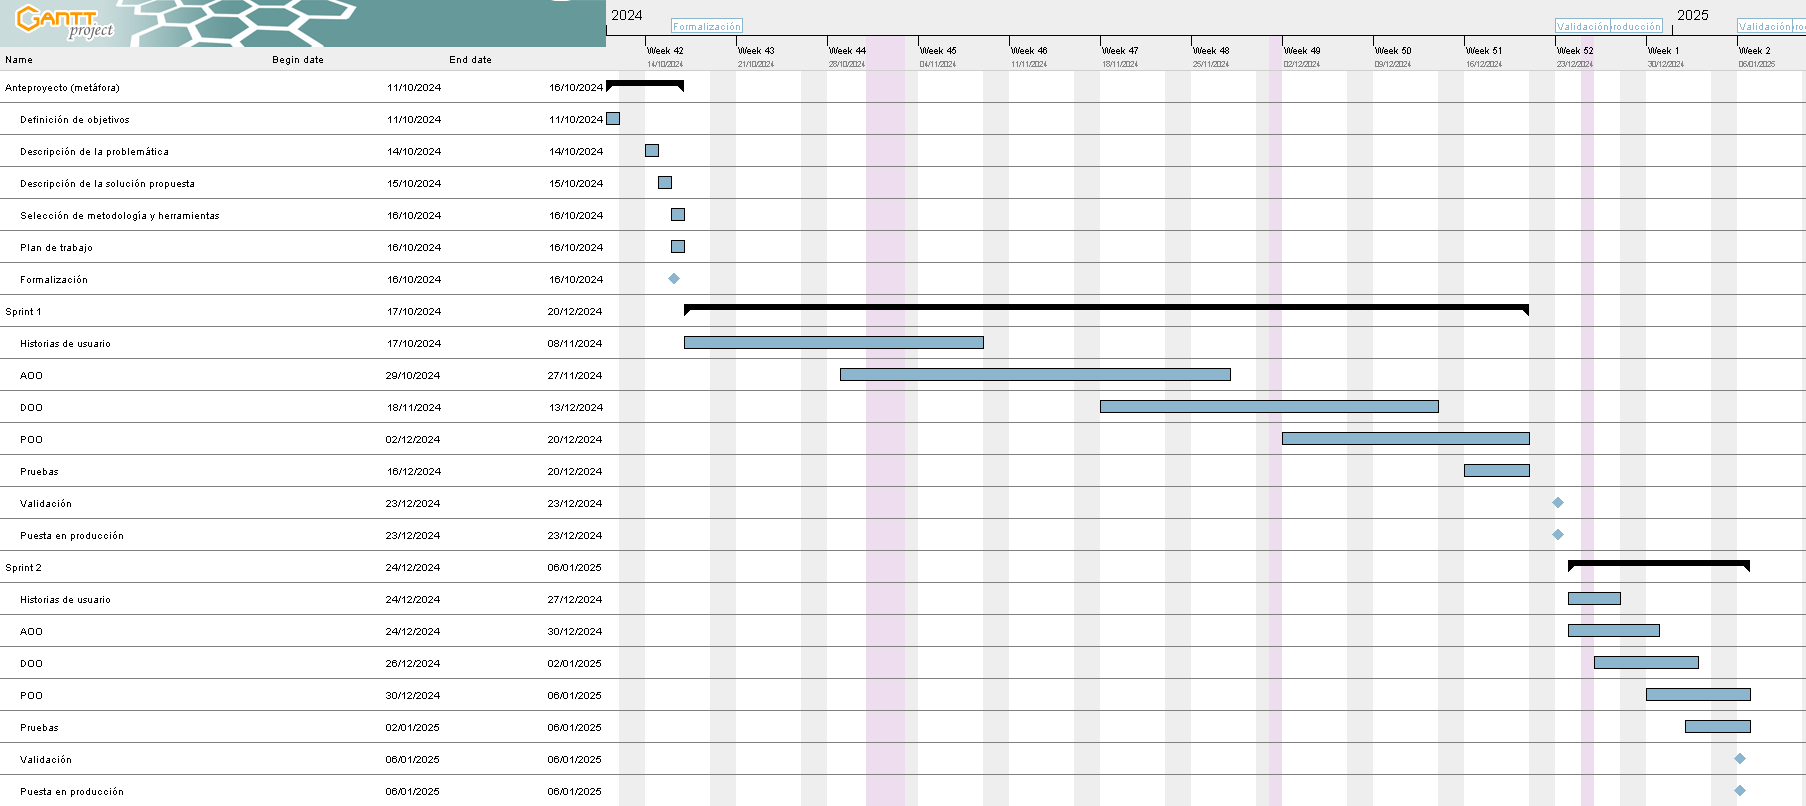
\includegraphics[width=\textwidth]{img/CartaGantt.png}
	\caption{Carta Gantt}
	\label{fig:CartaGantt}
\end{figure}
\clearpage

\section{Conclusiones}
El proyecto detallado en este informe tiene como objetivo el desarrollo de una aplicación móvil de alarmas para la plataforma Android. Para esto, se definió claramente la metodología a usar, además de los hitos importantes que se consideran en la planificación. Se establecen las fechas de dichos hitos a través de una carta Gantt, además de los recursos humanos y tecnologías que serán utilizadas para su desarrollo.
\\\\
El trabajo se realizó de manera híbrida, trabajando tanto de forma prescencial en la universidad, como a través de medios digitales. Habiendo dado término a esta etapa del proyecto, el equipo se encuentra preparado para comenzar la siguiente etapa de ``Análisis de requerimientos y casos de uso".

\clearpage



\end{document}
